\documentclass[10pt,twocolumn]{article}
\usepackage{times}
\usepackage[pdftex]{graphicx}
\graphicspath{{./}{figs/}}

\begin{document}
\title{Artificial Life Creation Comparing Genetic Algorithms And Genetic Programming}
\author{Tom Cammann\\\\
Computer Science, cy004947@reading.ac.uk}
\date{}
\maketitle
\begin{abstract}
This report focuses on the generating artificial life through two distinct methods, genetic algorithms and genetic programming. The report describes the fundamentals of these two methodologies, compares and contrasts their differences in the creation of similar artificial life. The report outlines tools developed during this project to accomplish an effective comparison of these two methods. These include a method of visualising the artificial life and the environment it inhabits during its existence. The outcome of this project demonstrates how genetic programming requires more advanced programming but can lead to novel and emergent behaviour, in contrast to genetic algorithms which are much simpler and can better replicate biological processes that go on around us. 
\end{abstract}


\section{INTRODUCTION}

Artificial life or ALife is the study and implementation of systems that are simulations or replications of natural life.
These systems can be biochemical, mechanical, computer software and many other medium that supports the existence of structured self controlled information.
This report will be looking at software artificial life, or Soft ALife and how it can be implemented using evolutionary computation.
Evolutionary computation has been used for the creation of artificial life for many decades, REF + EXAMPLE.
Using evolutionary computation has many qualities that replicate naturally evolved life, and is one few computational methods known that can generate solutions to problems without human interaction.
Evolutionary computation has been applied to artificial life to generate life forms that can inhabit an environment and are 'solutions' to this environment.

\paragraph{}
Evolutionary computation generally works by generating a population of solutions to a problem, and then using this population to create a better next population that can solve the given problem better.
To create a better population crossover, mutation and selection are used in various forms to generate a fitter population.
Each of these populations is referred to as a generation.
Each member in the population is a solution to the problem, however these solutions do not have to be correct, and are often close to correct before many generations have passed.
Each member of the population is assigned a fitness value to correspond with how close the solution is to correct, or how effective the solution is.
In the Context of artificial life this fitness value may correspond to how well the life form survives in a given environment.

% why are we comparing these 2 methods
\paragraph{}
The purpose of this investigation is to compare and contrast the usage of genetic algorithms and genetic programming in the creation of artificial life. Genetic programming first became prevelvant in the early 1990 after Koza used used GP to solve ??? ~\cite{Koza90}. After the advancements made by Koza many applications for GP emerged and one of the earlier appications was in ALife. Before these advancements GA was the primary method for generating ALife.

However these two have very different implementations and usage, this report will investigate the usage of both in the context of artificial life creation. 
% Genetic programming can generate unique solutions, unrestrained, GA more restrained. 

\paragraph{}
%how we compare them



\section{GENETIC ALGORITHMS}

Genetic algorithms were first designed and implemented by ??? in ??? when ???.

The general form of a genetic algorithm uses genes to represent parameters inside a program.
These parameters effect the running of a program.
These genes were historically represented in binary form, however more modern implementations can use any value as a gene, from programming objects to double floating point numbers.
These genes must be able to mutate, this is easy to understand when using binary number, to mutate a binary number you flip one bit in the gene sequence. 

\subsection{POPULATION REPRESENTATION}
In genetic algorithms each member of the population (or candidate solution) is represented by a list or string of values.
Each value represents a parameter that will be used in the solution.
The value could represent the number of iterations of a loop or represent a operator in a sum.
Traditionally binary numbers strings were used to represent a member of the population.
This was because of the ease of which this could be manipulated by computers and the simplicity mutations could be achieved.
To mutate a binary string a bit can be flipped.
This can work in most situations however it soon becomes apparent that this cannot useful in all situations.
%Fix and show formula? Find solutin.
If numbers are being represented in binary strings the most significant bit is at start of the string, if this is flipped then the number will change by a factor of ???.


\subsection{MUTATION}
In genetic algorithms mutation occurs on a per gene basis. If a mutation for a population member is needed then a gene in that~\cite{j1}. 

%better title needed!!!
%Section about how this project uses GA
\subsection{USAGE IN THIS}

\section{GENETIC PROGRAMMING}
%intro to gp

\subsection{POPULATION REPRESENTATION}
%obv

\subsection{MUTATION}
%asdsss



\section{SIMULATION}
To evaluate a common artificial life form a simulation environment has been created. This environment is a 2D arena where a life form must continue to consume food to survive, the more food the life form consumes the fitter the  



%talking about how the project framework
%how a frame to accommodate genetic programming and GA
\subsection{EVOLUTIONARY FRAMEWORK}
To investigate and compare these two algorithms %? algorithms??%
a framework to accommodate both algorithms was produced.  



\begin{figure} [ht]
\centering
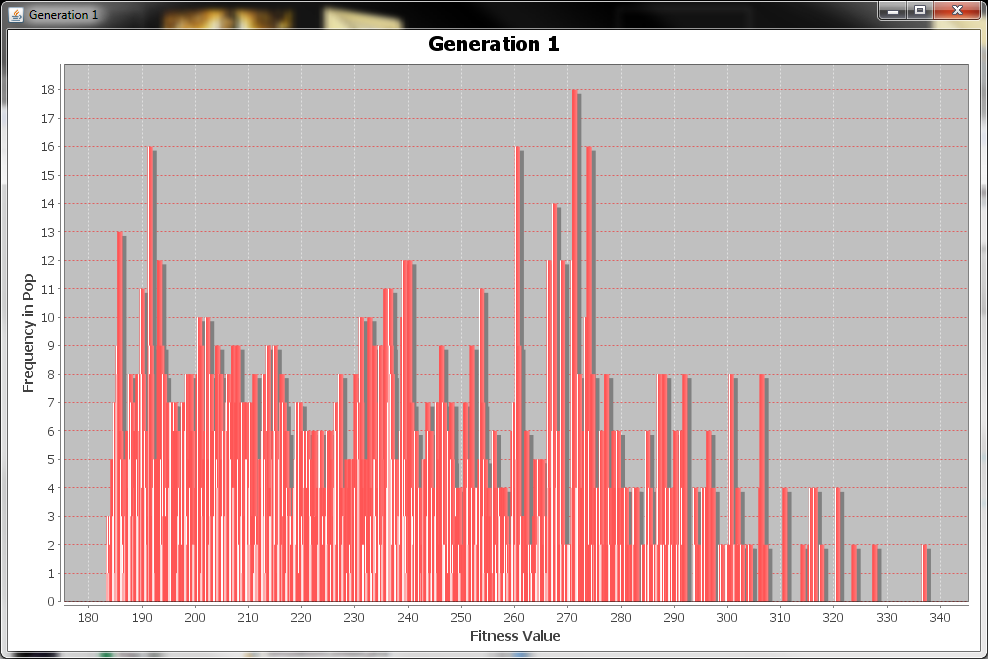
\includegraphics[scale = 0.25]{gen1-2500.png}
\caption{My figure}
\label{the-label-for-cross-referencing}
\end{figure}


\bibliographystyle{plain}
\bibliography{dis}

\end{document}
